\subsection{Experimental Evaluation}

The proposed gesture-based home automation system was evaluated in a controlled environment to assess its performance and effectiveness. The experiments were conducted in a room with dimensions of 380 cm (width) × 350 cm (height) × 450 cm (length) in which it performed well.

\subsubsection{Inference Time}
We measured the average inference time for various components of our system:

\begin{figure}[H]
	\centering
	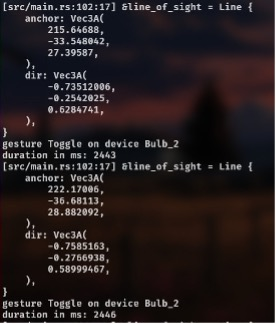
\includegraphics[scale=0.7]{images/inference_time_result.jpg} \\
	\caption{Code output with response time }
	\label{fig: Code output with response time }
\end{figure}

\begin{enumerate}
	\item \textbf{Gesture Identification \& Head Detection:} The gesture identification module, which utilizes the Mediapipe Pose Landmark model and an Artificial Neural Network (ANN), achieved an average inference time of 150 milliseconds per frame, The Head Detection module, which only utilized the mediapipe pose landmark model on frame from camera 2, achieved an average inference time of 100 milliseconds per frame. Both these modules run in parallel, so net latency is 150ms.
	\item \textbf{Head Pose Estimation:} The DirectMHP algorithm demonstrated an average inference time of 2250 milliseconds per frame.
	\item \textbf{3D User Positioning:} The depth-based 3D positioning module, which triangulates the user's coordinates using the two-camera setup, exhibited an average inference time of 2-5 milliseconds per frame.
	      But as this runs in parallel with Head Pose Estimation, this doesn't contribute to total response time.
\end{enumerate}

The overall end-to-end (from capturing frames to sending control signals to devices) average response time if a gesture was detected approximately 2400 milliseconds per frame. If gesture was not detected, the latency in capturing the next frame is 150

This result indicates that our system can operate in real-time, providing a responsive and seamless experience for users.



\begin{table}[h!]
	\centering
	\caption{Summary of Module Inference Times and Contribution to Latency}
	\resizebox{0.5\textwidth}{!}{%
		\begin{tabular}{|p{4cm}|p{5cm}|p{4cm}|p{3cm}|}
			\hline
			\textbf{Module}                & \textbf{Methodology/Model Used}                                 & \textbf{Average Inference Time (ms/frame)} & \textbf{Contribution to Total Latency}                             \\ \hline
			Gesture Identification         & Mediapipe Pose Landmark model + Artificial Neural Network (ANN) & 150                                        & 150 ms                                                             \\ \hline
			Head Detection                 & Mediapipe Pose Landmark model (camera 2)                        & 100                                        & Runs in parallel with Gesture Identification (150 ms)              \\ \hline
			Head Pose Estimation           & DirectMHP algorithm                                             & 2250                                       & Adds to total latency                                              \\ \hline
			3D User Positioning            & Depth-based triangulation using two-camera setup                & 2-5                                        & Runs in parallel with Head Pose Estimation (no additional latency) \\ \hline
			\textbf{Overall Response Time} & From frame capture to device control signal if gesture detected & \textbf{2400}                              &                                                                    \\ \hline
			\textbf{Latency (No Gesture)}  & Capture next frame latency                                      & \textbf{150}                               &                                                                    \\ \hline
		\end{tabular}%
	}
\end{table}


\subsubsection{Camera Calibration}

\paragraph{Root Mean Square Error (RMSE)}
The RMSE value obtained from the OpenCV \texttt{cv2.calibrateCamera()} function is provided. Lower RMSE suggesting a better alignment between the projected points and the observed points in the image.

\begin{equation}
	\text{RMSE} = 0.7
\end{equation}

Below are some sample images showing the annotated checkerboard pattern used for calibration. The detected corners are highlighted to illustrate the accuracy of the corner detection process.

% Insert images of checkerboard pattern here
\begin{figure}[h!]
	\centering
	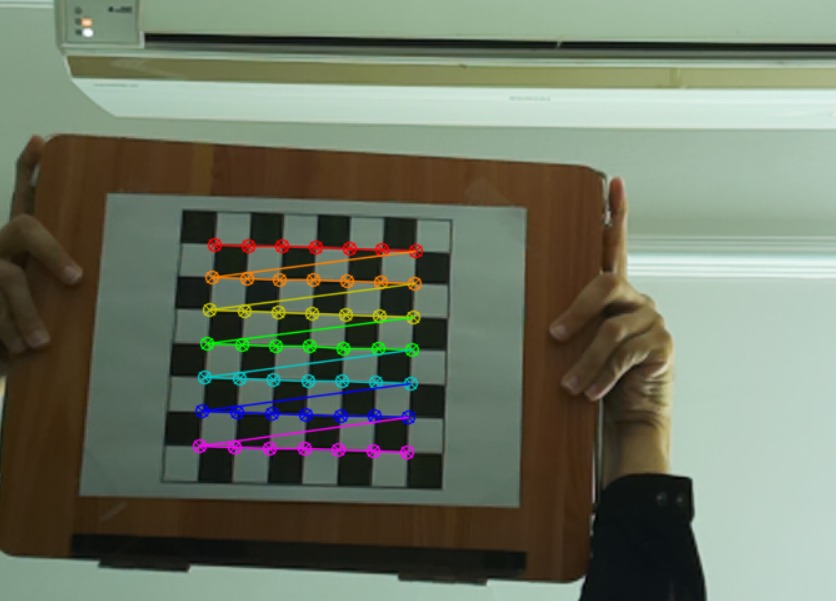
\includegraphics[height=0.2\textheight]{images/checkerboardL.jpeg}
	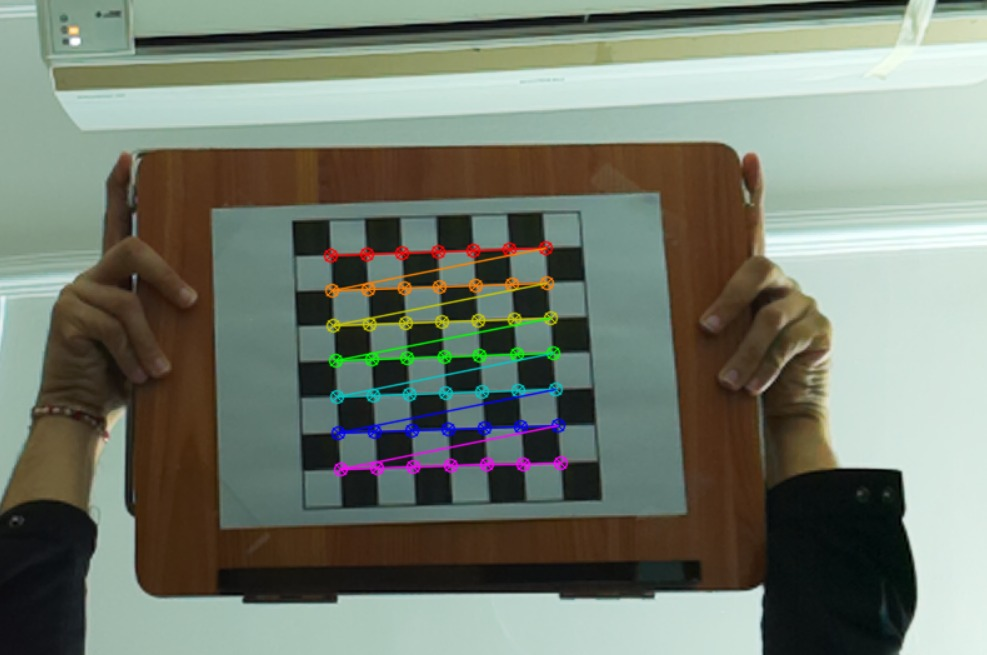
\includegraphics[height=0.2\textheight]{images/checkerboardR.jpeg}
	\caption{Annotated checkerboard pattern images showing detected corners.}
\end{figure}

\paragraph{Intrinsic Matrices of Cameras, Rotation and Translation Matrix of Camera 2 with Respect to Camera 1}
The intrinsic matrices for each camera, which include the focal lengths (\(f_x\), \(f_y\)) and the principal points (\(c_x\), \(c_y\)), Rotation matrix \(\mathbf{R}\) and Translation vector \(\mathbf{T}\) describe the position and orientation of Camera 2 relative to Camera 1 are shown below.


\begin{figure}[h!]
	\centering
	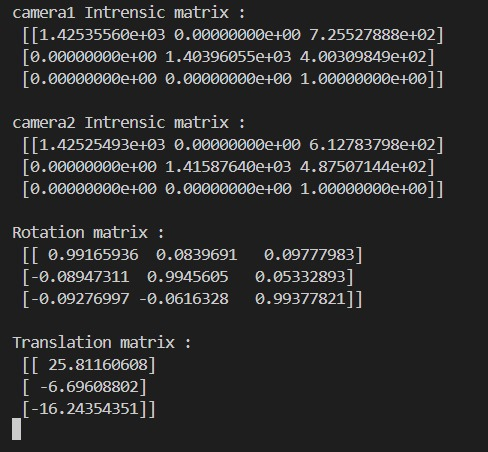
\includegraphics[height=0.4\textheight]{images/calibratiion_result.jpeg}
	\caption{Summary of Calibration Result}
\end{figure}


% The rotation matrix \(\mathbf{R}\) and translation vector \(\mathbf{T}\) describe the position and orientation of Camera 2 relative to Camera 1.


\subsubsection{Pose Landmark Estimation Models}


\subsubsection{Gesture Recognition Accuracy}
We evaluated our system's gesture recognition performance using a diverse dataset of hand and arm gestures. Our system achieved an overall gesture recognition accuracy of 98.4\%, demonstrating its robustness in identifying various gestures performed by users within the specified room dimensions.

The model is able to identify gestures as well as the LOS even if the person is facing opposite to the camera's direction.

For this system, we opted to use static gestures instead of dynamic gestures. Static gestures, such as hand raises, hand waves, and pointing motions, are faster to detect, more accurate, and less resource-intensive than dynamic gestures, which involve continuous movement. This choice was made to optimize the system's performance and responsiveness while minimizing computational requirements.

\subsubsection{3D Positioning Accuracy}
Precise 3D positioning is critical for correlating the user's gestures and head pose with the appropriate appliance in the room. Our system's depth-based 3D positioning module demonstrated an average deviation from the ground truth user position within the specified room dimensions as follows:

\begin{table}[h]
	\centering
	\begin{tabular}{|c|c|}
		\hline
		Axis & Deviation \\
		\hline
		x    & $\pm$5cm  \\
		y    & $\pm$5cm  \\
		z    & $\pm$10cm \\
		\hline
	\end{tabular}
\end{table}

\subsubsection{Sources of Measurement Error}

\begin{enumerate}
	\item \textbf{Field of View (FOV) Discrepancies:} One significant factor contributing to measurement inaccuracies is the discrepancy between the actual and specified field of view (FOV) of the cameras. Despite manufacturer specifications, the observed FOV may deviate, leading to distortions in perspective and subsequent errors in coordinate estimation.

	\item \textbf{Camera Orientation:} Misalignment in the orientation of the cameras, particularly in relation to the intended upright and horizontal positioning, was identified as another potential source of error. Even slight deviations from the optimal alignment can introduce systematic errors in the measured coordinates.

	\item \textbf{Stereo Vision Challenges:} The stereo correspondence process, fundamental to triangulating 3D coordinates from the images captured by both cameras, presents inherent challenges. Inaccuracies in matching corresponding image points between the stereo pair can result in erroneous depth estimations and subsequent errors in coordinate calculation.
\end{enumerate}
